

\documentclass[12pt]{article}
\usepackage{graphicx}
\usepackage{amsmath}
\usepackage{listings}
\usepackage{color}
\usepackage[section]{placeins} %this stops the figures from showing up in wrong section

\definecolor{dkgreen}{rgb}{0,0.6,0}
\definecolor{dkblue}{rgb}{0,0.0,0.6}
\definecolor{dkred}{rgb}{0.9,0.0,0.1}


\begin{document}

\lstset{language=Fortran,tabsize=4,numbers=left,numberstyle=\tiny,basicstyle=\ttfamily\small\color{dkblue},stringstyle=\ttfamily\color{blue},keywordstyle=\rmfamily\color{dkred}\bfseries\emph,backgroundcolor=\color{white},commentstyle=\color{dkgreen}}




\title{Physics 562 - Computational Physics\\[.5cm]
Assignment 3: Chaotic Double Pendulum}
\author{Josh Fernandes\\
Department of Physics \& Astronomy\\
California State University Long Beach}
\date{\today}

  
\maketitle



\begin{abstract}
This paper examine emergent chaos by analyzing a double pendulum. A double pendulum is a chaotic system that is nonlinear, deterministic, and highly sensitive to initial conditions. There are three states for the double pendulum to be in: no chaos, emerging chaos, and full chaos. These states correspond to a Lyapunov exponent that is negative, zero, and positive, respectively
\end{abstract}

\section{Single Pendulum}\label{s:intro}

A single pendulum is a very predictable system that undergoes simple harmonic motion. The kinetic energy of a pendulum is given by 

\begin{gather}
T=\frac{1}{2}mv^2=\frac{1}{2}m{(l\dot{\theta})}^2
\end{gather}
and the potential energy is given by

\begin{gather}
V=mgh=mgl(1 - cos(\theta))
\end{gather}
where $l$ is the length of the pendulum, and $m$ is the mass of the bob. The lagrangian is given by

\begin{gather}
\mathcal{L} = T - V = \frac{1}{2}m{(l\dot{\theta})}^2 - mgl(1 - cos(\theta)).
\end{gather}

The euler-lagrange equations can be applied to the lagrangian in order to get the equations of motions, but instead we will use the hamiltonian. The hamiltonian is given by

\begin{gather}
\mathcal{H} = \Sigma p_{q_i} \dot{q_i} - \mathcal{L} =p_{\theta}\dot{\theta} - \frac{1}{2}m{(l\dot{\theta})}^2 + mgl(1 - cos(\theta)).
\end{gather}
Furthurmore we know that

\begin{gather}
p_{\theta} = \frac{\partial \mathcal{L}}{\partial \theta} = ml^2\dot{\theta}
\end{gather}
which can be rewritten

\begin{gather}
\dot{\theta} = \frac{p_{\theta}}{ml^2}
\end{gather}
so we can substitute into the hamiltonian to get it of the form 

\begin{gather}
\mathcal{H} =\frac{p_{\theta}^2}{ml^2} - \frac{1}{2}ml^2{(\frac{p_{\theta}}{ml^2})}^2 + mgl(1 - cos(\theta)).  \\
\mathcal{H} =\frac{p_{\theta}^2}{ml^2} - \frac{1}{2}{\frac{p_{\theta}^2}{ml^2}} + mgl(1 - cos(\theta)). \\
\mathcal{H} =\frac{1}{2}{\frac{p_{\theta}^2}{ml^2}} + mgl(1 - cos(\theta)).
\end{gather}
We can then solve the hamiltonian equations of motion which are

\begin{gather}
\dot{\theta} = \frac{\partial \mathcal{H}}{\partial p_{\theta}} = \frac{p_{\theta}}{ml^2} \\
\dot{p_{\theta}} = -\frac{\partial \mathcal{H}}{\partial \theta} = -mgl sin{\theta}
\end{gather}


\section{Double Pendulum}

The double pendulum is more complex. The equations of motion for the double pendulum is given by

\begin{gather}
\dot{\theta_1} = \frac{\partial \mathcal{H}}{\partial p_{1}} = \frac{lp_1-lp_2cos(\theta_1-\theta_2)}{l^3[m_1+m_2sin^2(\theta_1-\theta_2)]} \\
\dot{\theta_2} = \frac{\partial \mathcal{H}}{\partial p_{2}} = \frac{l(m_1+m_2)p_2-lm_2p_1cos(\theta_1-\theta_2)}{l^3m_2[m_1+m_2sin^2(\theta_1-\theta_2)]} \\
\dot{p_1} = -\frac{\partial \mathcal{H}}{\partial \theta_1} = -(m_1+m_2)glsin(\theta_1) - C_1 + C_2 \\
\dot{p_2} = -\frac{\partial \mathcal{H}}{\partial \theta_2} = -m_2glsin(\theta_2) + C_1 - C_2
\end{gather}

where

\begin{gather}
C_1 \equiv \frac{p_1p_2sin(\theta_1-\theta_2)}{l^2[m_1+m_2sin^2(\theta_1-\theta_2)]} \\
C_2 \equiv \frac{l^2m_2p_1^2+l^2(m_1+m_2)p_2^2-l^2m_2p_1p_2cos(\theta_1-\theta_2)}{2l^4[m_1+m_2sin^2(\theta_1-\theta_2)]^2}sin[2(\theta_1-\theta_2)]
\end{gather}
In order to understand how the double pendulum behaves, the momentum will be plotted against the angle for each pendulum. In addition, the lyapunov exponent will be calculated for three different cases. These cases are 

\begin{lstlisting}[frame=single,caption={Module {\tt Cases}},label=module]

	!!Low Energy - No Chaos
	y(1) = 1._dp*(pi/180)			! initial angle for 1st pendulum
	y(2) = 0._dp				! initial momentum for 1st pendulum
	y(3) = 1._dp*(pi/180)			! initial angle for 2nd pendulum
	y(4) = 0._dp				! initial momentum for 2nd pendulum

	!!Medium Energy - Emerging Chaos But Stable Orbit
 	y(1) = 1._dp*(pi/180)			! initial angle for 1st pendulum
 	y(2) = 1._dp				! initial momentum for 1st pendulum
  	y(3) = 1._dp*(pi/180)			! initial angle for 2nd pendulum
  	y(4) = 1.01_dp				! initial momentum for 2nd pendulum

	!!High Energy - Full Chaos
 	y(1) = 1._dp*(pi/180)			! initial angle for 1st pendulum
 	y(2) = 1._dp				! initial momentum for 1st pendulum
 	y(3) = 1._dp*(pi/180)			! initial angle for 2nd pendulum
 	y(4) = 1.3_dp				! initial momentum for 2nd pendulum

\end{lstlisting}
The mass for the first bob is 1 kg and the mass of the second bob is 2 kg. The length of both pendulums is 1 meter. The lyapunov exponents are given by
\begin{gather}
|p_1-p_2|=e^{\lambda \cdot t}
\end{gather}
where $P_1$ and $p_2$ are the momenta for the two pendulums, and $\lambda$ is the lyapunov exponent.

\section{The Fortran95 code}

The code solves the equation of motion using the Runga-Kutta method. First a module called {\tt NumType} is created to store all my global parameters.
\begin{lstlisting}[frame=single,caption={Module {\tt NumType}},label=module]

module NumType

	save
	integer, parameter :: dp = kind(1.d0)
	real(dp), parameter :: pi = 4*atan(1._dp), &
	e = exp(1._dp)
	complex(dp), parameter :: iic = (0._dp,1._dp)
	
end module NumType

\end{lstlisting}

\begin{lstlisting}[frame=single,caption={ {\tt rkf45.f95}},label=module]

subroutine rkf45step(t,y,h)  ! 4-th order Runge-Kutta step
	
	use setup, only : dp, n_eq
	implicit none
	real(dp), intent(inout) :: t, h
	real(dp), dimension(n_eq), intent(inout) :: y 
	real(dp), dimension(n_eq) :: k1, k2, k3, k4, k5, k6, y1, y2
	real(dp), parameter :: epsilon = 1.e-6_dp, tiny = 1.e-20_dp
	real(dp) :: rr, delta
		
	call deriv(t,	     h,	 y,	   k1)
	call deriv(t+h/4,	 h,  y+ k1/4,   k2)
	call deriv(t+3*h/8,	 h,  y+ (3*k1+9*k2)/32,  k3)
	call deriv(t+12*h/13,h,	 y+ (1932*k1-7200*k2+7296*k3) &
	/2197 , k4)	
	call deriv(t+h,	     h,  y+ (439*k1/216-8*k2+3680*k3/513 &
	-845*k4/4104),	  k5)	
	call deriv(t+h/2,	 h,  y+ (-8*k1/27 +2*k2-3544*k3/2565 + &
	1859*k4/4104 -11*k5/40),	k6)
	
    y1 = y + 25*k1/216 + 1408*k3/2565 + 2197*k4/4104 &
     - k5/5
    y2 = y + 16*k1/135 + 6656*k3/12825 + 28561*k4/ & 
    56430 - 9*k5/50 + 2*k6/55
    
   rr = sqrt(dot_product(y1-y2,y1-y2))/h + tiny
    
    if ( rr < epsilon ) then
        t = t + h
        y = y1
        delta = 0.92_dp * (epsilon/rr)**(0.2_dp)
        h = delta*h
        write (unit = 3,fmt='(3f20.10)') t, y(1)
        write (unit = 4,fmt='(3f20.10)') t, y(2)
        write (unit = 5,fmt='(3f20.10)') t, y(3)
        write (unit = 6,fmt='(3f20.10)') t, y(4)
        write (unit = 7,fmt='(3f20.10)') y(1), y(2)
        write (unit = 8,fmt='(3f20.10)') y(3), y(4)
        write (unit = 9,fmt='(3f20.10)') -sin(y(1)),-cos(y(1))
        write (unit = 10,fmt='(3f20.10)') -sin(y(1))-sin(y(3)) &
        ,-cos(y(1))-cos(y(3))
    else
        delta = 0.92_dp * (epsilon/rr)**(0.25_dp)
        h = delta*h
    end if
	
    	
    contains
    
        subroutine deriv(t,h,y,k)   ! derivative

	        use setup, only : dp, n_eq, g, length, mass1, mass2
	        implicit none
	        real(dp), intent(in) :: t, h
	        real(dp), dimension(n_eq), intent(in) :: y
	        real(dp), dimension(n_eq) :: f, k
	        real(dp) :: c1, c2

	        c1 = (y(2)*y(4)*sin(y(1)-y(3)))/ &
	        	(length*length*(mass1+mass2*(sin(y(1)-y(3)))**2))
	        c2 = (length**2*mass2*y(2)**2 + &
				length**2*(mass1+mass2)*y(4)**2- &
				length*length*mass2*y(2)*y(4)*cos(y(1)-y(3)))/ &
				(2*length**4*(mass1+mass2*(sin(y(1)-y(3)))**2)**2)* &
				sin(2*(y(1)-y(3)))

			f(1) = (length*y(2) - length*y(4)*cos(y(1)-y(2)))/ &
					(length**3*(mass1+mass2*(sin(y(1)-y(2)))**2))
			f(2) = -(mass1+mass2)*g*length*sin(y(1)) - c1 + c2
			f(3) = (length*(mass1+mass2)*y(4) - length*&
					mass2*y(2)*cos(y(1)-y(2)))/ &
					(length**3*mass2*(mass1+mass2*(sin(y(1)-y(2)))**2))
			f(4) = -mass2*g*length*sin(y(3)) + c1 - c2
	        
	        k(1:n_eq) = h*f(1:n_eq)
	        
        end subroutine deriv


\end{lstlisting}

The main program is {\tt adpend} and it begins with its own module. 

\begin{lstlisting}[frame=single,caption={{\tt adpend.f95}},label=adpend]


module setup

	use NumType
	implicit none
	integer, parameter :: n_eq = 4
	real(dp), parameter:: g = 10.0_dp, length = 1.0_dp, &
	 mass1 = 1.0_dp, mass2 = 2.0_dp
	real(dp) :: t, tmax, dt, lambda
	real(dp), dimension(n_eq) :: y
	
end module setup

program pendulum

	use setup
	implicit none

	!!initial conditions!!
		
	t = 0._dp					! time to start
	tmax = 100._dp				! time to exit
	dt = 0.001_dp				! time step
	lambda = 0._dp				!intiate a value for lyapanov exponent


	!!Below are four cases - Make sure only one set of y is uncommented!!

	!!Low Energy - No Chaos
	y(1) = 1._dp*(pi/180)		! initial angle 1
	y(2) = 0._dp				! initial momentum 1
	y(3) = 1._dp*(pi/180)		! initial angle 2
	y(4) = 0._dp				! initial momentum 2

	!!Medium Energy - Emerging Chaos But Stable Orbit
!  	y(1) = 1._dp*(pi/180)		! initial angle 1
!  	y(2) = 1._dp				! initial momentum 1
!  	y(3) = 1._dp*(pi/180)		! initial angle 2
!  	y(4) = 1.01_dp				! initial momentum 2

	!!High Energy - Full Chaos
! 	y(1) = 1._dp*(pi/180)		! initial angle 1
! 	y(2) = 1._dp				! initial momentum 1
! 	y(3) = 1._dp*(pi/180)		! initial angle 2
! 	y(4) = 1.3_dp				! initial momentum 2

	!!High Energy - Full Chaos
! 	y(1) = 60._dp*(pi/180)		! initial angle 1
! 	y(2) = 1._dp				! initial momentum 1
! 	y(3) = 60._dp*(pi/180)		! initial angle 2
! 	y(4) = 2._dp				! initial momentum 2

	
	!!open all the files that data will be written to!!

	open(unit = 3, file = 'pend_angle1.data', &
	    action = 'write', status = 'replace')
	open(unit = 4, file = 'pend_mom1.data', &
	    action = 'write', status = 'replace')
	open(unit = 5, file = 'pend_angle2.data', &
	    action = 'write', status = 'replace')
	open(unit = 6, file = 'pend_mom2.data', &
	    action = 'write', status = 'replace')
	open(unit = 7, file = 'angle_mom1.data', &
	    action = 'write', status = 'replace')
	open(unit = 8, file = 'angle_mom2.data', &
	    action = 'write', status = 'replace')
	open(unit = 9, file = 'pend_xy1.data', &
	    action = 'write', status = 'replace')
	open(unit = 10, file = 'pend_xy2.data', &
	    action = 'write', status = 'replace')
	open(unit = 11, file = 'lambda.data', &
	    action = 'write', status = 'replace')

	!!calculate the momenta and angle of the pendulums!!

	do while ( t < tmax )
		if ( t + dt > tmax) dt = tmax -t
		call rkf45step(t,y,dt)						
		!use the runga kutta method to calculate for theta and momentum
		lambda = lambda + log(abs(y(4)-y(2)))/t 	
		!update the summation of the lyapanov exponent
		write (unit = 11,fmt='(3f20.10)') lambda 	
		!write lamba to file
	end do

end program pendulum

\end{lstlisting}


The code is run by typing {\tt ./pend}. Various data sets are plotted to different files for easy graphing.
\section{Results}

A single pendulum is very ordered and predictable.  

\begin {figure}[!htb]
	\resizebox{\columnwidth}{!}{% GNUPLOT: LaTeX picture with Postscript
\begingroup
  \makeatletter
  \providecommand\color[2][]{%
    \GenericError{(gnuplot) \space\space\space\@spaces}{%
      Package color not loaded in conjunction with
      terminal option `colourtext'%
    }{See the gnuplot documentation for explanation.%
    }{Either use 'blacktext' in gnuplot or load the package
      color.sty in LaTeX.}%
    \renewcommand\color[2][]{}%
  }%
  \providecommand\includegraphics[2][]{%
    \GenericError{(gnuplot) \space\space\space\@spaces}{%
      Package graphicx or graphics not loaded%
    }{See the gnuplot documentation for explanation.%
    }{The gnuplot epslatex terminal needs graphicx.sty or graphics.sty.}%
    \renewcommand\includegraphics[2][]{}%
  }%
  \providecommand\rotatebox[2]{#2}%
  \@ifundefined{ifGPcolor}{%
    \newif\ifGPcolor
    \GPcolortrue
  }{}%
  \@ifundefined{ifGPblacktext}{%
    \newif\ifGPblacktext
    \GPblacktexttrue
  }{}%
  % define a \g@addto@macro without @ in the name:
  \let\gplgaddtomacro\g@addto@macro
  % define empty templates for all commands taking text:
  \gdef\gplbacktext{}%
  \gdef\gplfronttext{}%
  \makeatother
  \ifGPblacktext
    % no textcolor at all
    \def\colorrgb#1{}%
    \def\colorgray#1{}%
  \else
    % gray or color?
    \ifGPcolor
      \def\colorrgb#1{\color[rgb]{#1}}%
      \def\colorgray#1{\color[gray]{#1}}%
      \expandafter\def\csname LTw\endcsname{\color{white}}%
      \expandafter\def\csname LTb\endcsname{\color{black}}%
      \expandafter\def\csname LTa\endcsname{\color{black}}%
      \expandafter\def\csname LT0\endcsname{\color[rgb]{1,0,0}}%
      \expandafter\def\csname LT1\endcsname{\color[rgb]{0,1,0}}%
      \expandafter\def\csname LT2\endcsname{\color[rgb]{0,0,1}}%
      \expandafter\def\csname LT3\endcsname{\color[rgb]{1,0,1}}%
      \expandafter\def\csname LT4\endcsname{\color[rgb]{0,1,1}}%
      \expandafter\def\csname LT5\endcsname{\color[rgb]{1,1,0}}%
      \expandafter\def\csname LT6\endcsname{\color[rgb]{0,0,0}}%
      \expandafter\def\csname LT7\endcsname{\color[rgb]{1,0.3,0}}%
      \expandafter\def\csname LT8\endcsname{\color[rgb]{0.5,0.5,0.5}}%
    \else
      % gray
      \def\colorrgb#1{\color{black}}%
      \def\colorgray#1{\color[gray]{#1}}%
      \expandafter\def\csname LTw\endcsname{\color{white}}%
      \expandafter\def\csname LTb\endcsname{\color{black}}%
      \expandafter\def\csname LTa\endcsname{\color{black}}%
      \expandafter\def\csname LT0\endcsname{\color{black}}%
      \expandafter\def\csname LT1\endcsname{\color{black}}%
      \expandafter\def\csname LT2\endcsname{\color{black}}%
      \expandafter\def\csname LT3\endcsname{\color{black}}%
      \expandafter\def\csname LT4\endcsname{\color{black}}%
      \expandafter\def\csname LT5\endcsname{\color{black}}%
      \expandafter\def\csname LT6\endcsname{\color{black}}%
      \expandafter\def\csname LT7\endcsname{\color{black}}%
      \expandafter\def\csname LT8\endcsname{\color{black}}%
    \fi
  \fi
  \setlength{\unitlength}{0.0500bp}%
  \begin{picture}(7200.00,5040.00)%
    \gplgaddtomacro\gplbacktext{%
      \csname LTb\endcsname%
      \put(814,704){\makebox(0,0)[r]{\strut{}$-60$}}%
      \csname LTb\endcsname%
      \put(814,1317){\makebox(0,0)[r]{\strut{}$-40$}}%
      \csname LTb\endcsname%
      \put(814,1929){\makebox(0,0)[r]{\strut{}$-20$}}%
      \csname LTb\endcsname%
      \put(814,2542){\makebox(0,0)[r]{\strut{}$0$}}%
      \csname LTb\endcsname%
      \put(814,3154){\makebox(0,0)[r]{\strut{}$20$}}%
      \csname LTb\endcsname%
      \put(814,3767){\makebox(0,0)[r]{\strut{}$40$}}%
      \csname LTb\endcsname%
      \put(814,4379){\makebox(0,0)[r]{\strut{}$60$}}%
      \csname LTb\endcsname%
      \put(946,484){\makebox(0,0){\strut{}$-0.6$}}%
      \csname LTb\endcsname%
      \put(1922,484){\makebox(0,0){\strut{}$-0.4$}}%
      \csname LTb\endcsname%
      \put(2898,484){\makebox(0,0){\strut{}$-0.2$}}%
      \csname LTb\endcsname%
      \put(3875,484){\makebox(0,0){\strut{}$0$}}%
      \csname LTb\endcsname%
      \put(4851,484){\makebox(0,0){\strut{}$0.2$}}%
      \csname LTb\endcsname%
      \put(5827,484){\makebox(0,0){\strut{}$0.4$}}%
      \csname LTb\endcsname%
      \put(6803,484){\makebox(0,0){\strut{}$0.6$}}%
      \put(176,2541){\rotatebox{-270}{\makebox(0,0){\strut{}$p_{\theta}$}}}%
      \put(3874,154){\makebox(0,0){\strut{}$\theta$}}%
      \put(3874,4709){\makebox(0,0){\strut{}single pendulum}}%
    }%
    \gplgaddtomacro\gplfronttext{%
      \csname LTb\endcsname%
      \put(5816,4206){\makebox(0,0)[r]{\strut{}plot}}%
    }%
    \gplbacktext
    \put(0,0){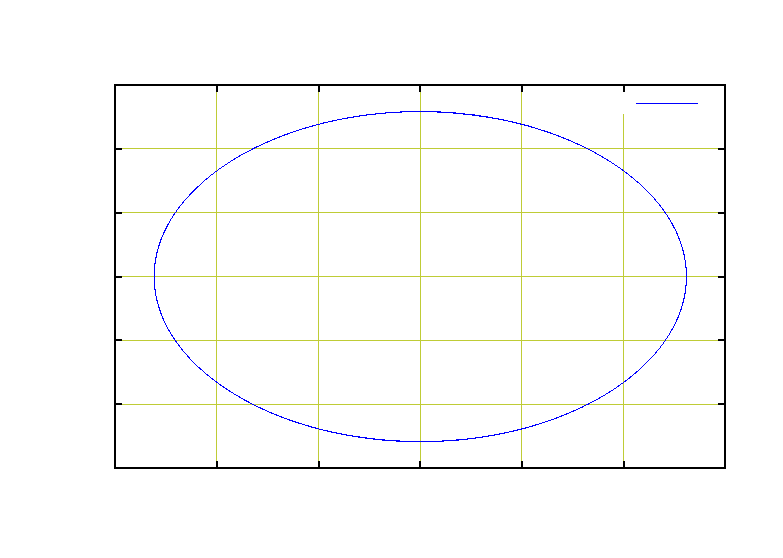
\includegraphics{eg1}}%
    \gplfronttext
  \end{picture}%
\endgroup
}
	\caption{A simple pendulum. }
	\label{singlependulum}
\end {figure}

Figure \ref{singlependulum} shows that you can predict the values of the momentum for any time $t$. The momentum is maximum when the pendulum is at the bottom of the arc and zero at the ends of the swing. Because of this, there is no chaos in the pendulums movement.

\begin {figure}[!htb]
	\resizebox{\columnwidth}{!}{% GNUPLOT: LaTeX picture with Postscript
\begingroup
  \makeatletter
  \providecommand\color[2][]{%
    \GenericError{(gnuplot) \space\space\space\@spaces}{%
      Package color not loaded in conjunction with
      terminal option `colourtext'%
    }{See the gnuplot documentation for explanation.%
    }{Either use 'blacktext' in gnuplot or load the package
      color.sty in LaTeX.}%
    \renewcommand\color[2][]{}%
  }%
  \providecommand\includegraphics[2][]{%
    \GenericError{(gnuplot) \space\space\space\@spaces}{%
      Package graphicx or graphics not loaded%
    }{See the gnuplot documentation for explanation.%
    }{The gnuplot epslatex terminal needs graphicx.sty or graphics.sty.}%
    \renewcommand\includegraphics[2][]{}%
  }%
  \providecommand\rotatebox[2]{#2}%
  \@ifundefined{ifGPcolor}{%
    \newif\ifGPcolor
    \GPcolortrue
  }{}%
  \@ifundefined{ifGPblacktext}{%
    \newif\ifGPblacktext
    \GPblacktexttrue
  }{}%
  % define a \g@addto@macro without @ in the name:
  \let\gplgaddtomacro\g@addto@macro
  % define empty templates for all commands taking text:
  \gdef\gplbacktext{}%
  \gdef\gplfronttext{}%
  \makeatother
  \ifGPblacktext
    % no textcolor at all
    \def\colorrgb#1{}%
    \def\colorgray#1{}%
  \else
    % gray or color?
    \ifGPcolor
      \def\colorrgb#1{\color[rgb]{#1}}%
      \def\colorgray#1{\color[gray]{#1}}%
      \expandafter\def\csname LTw\endcsname{\color{white}}%
      \expandafter\def\csname LTb\endcsname{\color{black}}%
      \expandafter\def\csname LTa\endcsname{\color{black}}%
      \expandafter\def\csname LT0\endcsname{\color[rgb]{1,0,0}}%
      \expandafter\def\csname LT1\endcsname{\color[rgb]{0,1,0}}%
      \expandafter\def\csname LT2\endcsname{\color[rgb]{0,0,1}}%
      \expandafter\def\csname LT3\endcsname{\color[rgb]{1,0,1}}%
      \expandafter\def\csname LT4\endcsname{\color[rgb]{0,1,1}}%
      \expandafter\def\csname LT5\endcsname{\color[rgb]{1,1,0}}%
      \expandafter\def\csname LT6\endcsname{\color[rgb]{0,0,0}}%
      \expandafter\def\csname LT7\endcsname{\color[rgb]{1,0.3,0}}%
      \expandafter\def\csname LT8\endcsname{\color[rgb]{0.5,0.5,0.5}}%
    \else
      % gray
      \def\colorrgb#1{\color{black}}%
      \def\colorgray#1{\color[gray]{#1}}%
      \expandafter\def\csname LTw\endcsname{\color{white}}%
      \expandafter\def\csname LTb\endcsname{\color{black}}%
      \expandafter\def\csname LTa\endcsname{\color{black}}%
      \expandafter\def\csname LT0\endcsname{\color{black}}%
      \expandafter\def\csname LT1\endcsname{\color{black}}%
      \expandafter\def\csname LT2\endcsname{\color{black}}%
      \expandafter\def\csname LT3\endcsname{\color{black}}%
      \expandafter\def\csname LT4\endcsname{\color{black}}%
      \expandafter\def\csname LT5\endcsname{\color{black}}%
      \expandafter\def\csname LT6\endcsname{\color{black}}%
      \expandafter\def\csname LT7\endcsname{\color{black}}%
      \expandafter\def\csname LT8\endcsname{\color{black}}%
    \fi
  \fi
  \setlength{\unitlength}{0.0500bp}%
  \begin{picture}(7200.00,5040.00)%
    \gplgaddtomacro\gplbacktext{%
      \csname LTb\endcsname%
      \put(1078,704){\makebox(0,0)[r]{\strut{}$-0.2$}}%
      \csname LTb\endcsname%
      \put(1078,1163){\makebox(0,0)[r]{\strut{}$-0.15$}}%
      \csname LTb\endcsname%
      \put(1078,1623){\makebox(0,0)[r]{\strut{}$-0.1$}}%
      \csname LTb\endcsname%
      \put(1078,2082){\makebox(0,0)[r]{\strut{}$-0.05$}}%
      \csname LTb\endcsname%
      \put(1078,2542){\makebox(0,0)[r]{\strut{}$0$}}%
      \csname LTb\endcsname%
      \put(1078,3001){\makebox(0,0)[r]{\strut{}$0.05$}}%
      \csname LTb\endcsname%
      \put(1078,3460){\makebox(0,0)[r]{\strut{}$0.1$}}%
      \csname LTb\endcsname%
      \put(1078,3920){\makebox(0,0)[r]{\strut{}$0.15$}}%
      \csname LTb\endcsname%
      \put(1078,4379){\makebox(0,0)[r]{\strut{}$0.2$}}%
      \csname LTb\endcsname%
      \put(1210,484){\makebox(0,0){\strut{}$-0.025$}}%
      \csname LTb\endcsname%
      \put(2329,484){\makebox(0,0){\strut{}$-0.015$}}%
      \csname LTb\endcsname%
      \put(3447,484){\makebox(0,0){\strut{}$-0.005$}}%
      \csname LTb\endcsname%
      \put(4566,484){\makebox(0,0){\strut{}$0.005$}}%
      \csname LTb\endcsname%
      \put(5684,484){\makebox(0,0){\strut{}$0.015$}}%
      \csname LTb\endcsname%
      \put(6803,484){\makebox(0,0){\strut{}$0.025$}}%
      \put(176,2541){\rotatebox{-270}{\makebox(0,0){\strut{}$p_{\theta_2}$}}}%
      \put(4006,154){\makebox(0,0){\strut{}$\theta_2$}}%
      \put(4006,4709){\makebox(0,0){\strut{}double pendulum - low energy}}%
    }%
    \gplgaddtomacro\gplfronttext{%
      \csname LTb\endcsname%
      \put(5816,4206){\makebox(0,0)[r]{\strut{}pendulum 2}}%
    }%
    \gplbacktext
    \put(0,0){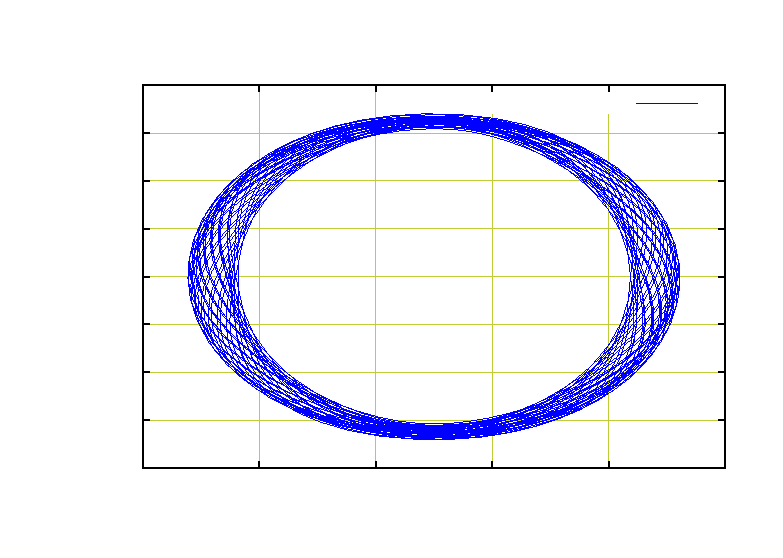
\includegraphics{eg2}}%
    \gplfronttext
  \end{picture}%
\endgroup
}
	\caption{Plot for the second bob. }
	\label{dobulepend1}
\end {figure}
Figure \ref{dobulepend1} is similar to the single pendulum. The orbit has slight variation but it is a stable orbit. The calculated lyapanov exponent is a negative number, which confirms that the orbit is closed. 

\begin {figure}[!htb]
	\resizebox{\columnwidth}{!}{% GNUPLOT: LaTeX picture with Postscript
\begingroup
  \makeatletter
  \providecommand\color[2][]{%
    \GenericError{(gnuplot) \space\space\space\@spaces}{%
      Package color not loaded in conjunction with
      terminal option `colourtext'%
    }{See the gnuplot documentation for explanation.%
    }{Either use 'blacktext' in gnuplot or load the package
      color.sty in LaTeX.}%
    \renewcommand\color[2][]{}%
  }%
  \providecommand\includegraphics[2][]{%
    \GenericError{(gnuplot) \space\space\space\@spaces}{%
      Package graphicx or graphics not loaded%
    }{See the gnuplot documentation for explanation.%
    }{The gnuplot epslatex terminal needs graphicx.sty or graphics.sty.}%
    \renewcommand\includegraphics[2][]{}%
  }%
  \providecommand\rotatebox[2]{#2}%
  \@ifundefined{ifGPcolor}{%
    \newif\ifGPcolor
    \GPcolortrue
  }{}%
  \@ifundefined{ifGPblacktext}{%
    \newif\ifGPblacktext
    \GPblacktexttrue
  }{}%
  % define a \g@addto@macro without @ in the name:
  \let\gplgaddtomacro\g@addto@macro
  % define empty templates for all commands taking text:
  \gdef\gplbacktext{}%
  \gdef\gplfronttext{}%
  \makeatother
  \ifGPblacktext
    % no textcolor at all
    \def\colorrgb#1{}%
    \def\colorgray#1{}%
  \else
    % gray or color?
    \ifGPcolor
      \def\colorrgb#1{\color[rgb]{#1}}%
      \def\colorgray#1{\color[gray]{#1}}%
      \expandafter\def\csname LTw\endcsname{\color{white}}%
      \expandafter\def\csname LTb\endcsname{\color{black}}%
      \expandafter\def\csname LTa\endcsname{\color{black}}%
      \expandafter\def\csname LT0\endcsname{\color[rgb]{1,0,0}}%
      \expandafter\def\csname LT1\endcsname{\color[rgb]{0,1,0}}%
      \expandafter\def\csname LT2\endcsname{\color[rgb]{0,0,1}}%
      \expandafter\def\csname LT3\endcsname{\color[rgb]{1,0,1}}%
      \expandafter\def\csname LT4\endcsname{\color[rgb]{0,1,1}}%
      \expandafter\def\csname LT5\endcsname{\color[rgb]{1,1,0}}%
      \expandafter\def\csname LT6\endcsname{\color[rgb]{0,0,0}}%
      \expandafter\def\csname LT7\endcsname{\color[rgb]{1,0.3,0}}%
      \expandafter\def\csname LT8\endcsname{\color[rgb]{0.5,0.5,0.5}}%
    \else
      % gray
      \def\colorrgb#1{\color{black}}%
      \def\colorgray#1{\color[gray]{#1}}%
      \expandafter\def\csname LTw\endcsname{\color{white}}%
      \expandafter\def\csname LTb\endcsname{\color{black}}%
      \expandafter\def\csname LTa\endcsname{\color{black}}%
      \expandafter\def\csname LT0\endcsname{\color{black}}%
      \expandafter\def\csname LT1\endcsname{\color{black}}%
      \expandafter\def\csname LT2\endcsname{\color{black}}%
      \expandafter\def\csname LT3\endcsname{\color{black}}%
      \expandafter\def\csname LT4\endcsname{\color{black}}%
      \expandafter\def\csname LT5\endcsname{\color{black}}%
      \expandafter\def\csname LT6\endcsname{\color{black}}%
      \expandafter\def\csname LT7\endcsname{\color{black}}%
      \expandafter\def\csname LT8\endcsname{\color{black}}%
    \fi
  \fi
  \setlength{\unitlength}{0.0500bp}%
  \begin{picture}(7200.00,5040.00)%
    \gplgaddtomacro\gplbacktext{%
      \csname LTb\endcsname%
      \put(946,704){\makebox(0,0)[r]{\strut{}$-1$}}%
      \csname LTb\endcsname%
      \put(946,1038){\makebox(0,0)[r]{\strut{}$-0.8$}}%
      \csname LTb\endcsname%
      \put(946,1372){\makebox(0,0)[r]{\strut{}$-0.6$}}%
      \csname LTb\endcsname%
      \put(946,1706){\makebox(0,0)[r]{\strut{}$-0.4$}}%
      \csname LTb\endcsname%
      \put(946,2040){\makebox(0,0)[r]{\strut{}$-0.2$}}%
      \csname LTb\endcsname%
      \put(946,2374){\makebox(0,0)[r]{\strut{}$0$}}%
      \csname LTb\endcsname%
      \put(946,2709){\makebox(0,0)[r]{\strut{}$0.2$}}%
      \csname LTb\endcsname%
      \put(946,3043){\makebox(0,0)[r]{\strut{}$0.4$}}%
      \csname LTb\endcsname%
      \put(946,3377){\makebox(0,0)[r]{\strut{}$0.6$}}%
      \csname LTb\endcsname%
      \put(946,3711){\makebox(0,0)[r]{\strut{}$0.8$}}%
      \csname LTb\endcsname%
      \put(946,4045){\makebox(0,0)[r]{\strut{}$1$}}%
      \csname LTb\endcsname%
      \put(946,4379){\makebox(0,0)[r]{\strut{}$1.2$}}%
      \csname LTb\endcsname%
      \put(1078,484){\makebox(0,0){\strut{}$-0.15$}}%
      \csname LTb\endcsname%
      \put(2032,484){\makebox(0,0){\strut{}$-0.1$}}%
      \csname LTb\endcsname%
      \put(2986,484){\makebox(0,0){\strut{}$-0.05$}}%
      \csname LTb\endcsname%
      \put(3941,484){\makebox(0,0){\strut{}$0$}}%
      \csname LTb\endcsname%
      \put(4895,484){\makebox(0,0){\strut{}$0.05$}}%
      \csname LTb\endcsname%
      \put(5849,484){\makebox(0,0){\strut{}$0.1$}}%
      \csname LTb\endcsname%
      \put(6803,484){\makebox(0,0){\strut{}$0.15$}}%
      \put(176,2541){\rotatebox{-270}{\makebox(0,0){\strut{}$p_{\theta_2}$}}}%
      \put(3940,154){\makebox(0,0){\strut{}$\theta_2$}}%
      \put(3940,4709){\makebox(0,0){\strut{}double pendulum - emerging chaos}}%
    }%
    \gplgaddtomacro\gplfronttext{%
      \csname LTb\endcsname%
      \put(5816,4206){\makebox(0,0)[r]{\strut{}pendulum 2}}%
    }%
    \gplbacktext
    \put(0,0){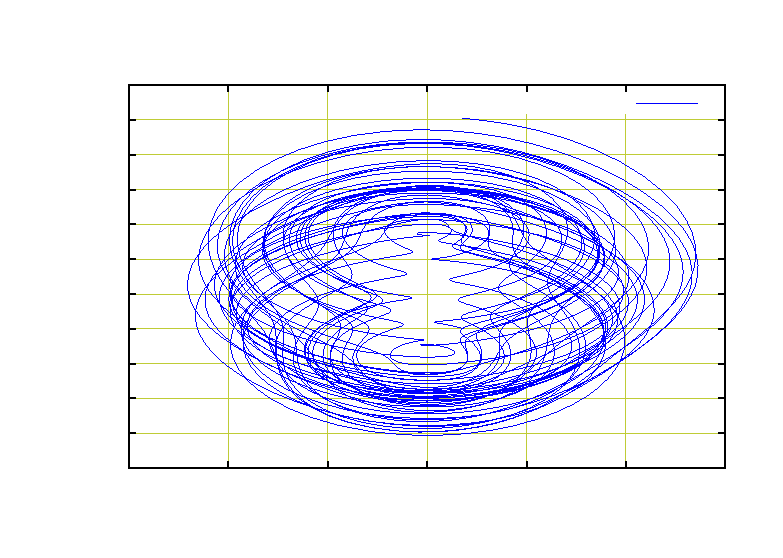
\includegraphics{eg3}}%
    \gplfronttext
  \end{picture}%
\endgroup
}
	\caption{The second bob begins to show chaotic motion, but resumes a stable orbit }
	\label{dobulepend2}
\end {figure}
Figure \ref{dobulepend2}

\begin {figure}[!htb]
	\resizebox{\columnwidth}{!}{% GNUPLOT: LaTeX picture with Postscript
\begingroup
  \makeatletter
  \providecommand\color[2][]{%
    \GenericError{(gnuplot) \space\space\space\@spaces}{%
      Package color not loaded in conjunction with
      terminal option `colourtext'%
    }{See the gnuplot documentation for explanation.%
    }{Either use 'blacktext' in gnuplot or load the package
      color.sty in LaTeX.}%
    \renewcommand\color[2][]{}%
  }%
  \providecommand\includegraphics[2][]{%
    \GenericError{(gnuplot) \space\space\space\@spaces}{%
      Package graphicx or graphics not loaded%
    }{See the gnuplot documentation for explanation.%
    }{The gnuplot epslatex terminal needs graphicx.sty or graphics.sty.}%
    \renewcommand\includegraphics[2][]{}%
  }%
  \providecommand\rotatebox[2]{#2}%
  \@ifundefined{ifGPcolor}{%
    \newif\ifGPcolor
    \GPcolortrue
  }{}%
  \@ifundefined{ifGPblacktext}{%
    \newif\ifGPblacktext
    \GPblacktexttrue
  }{}%
  % define a \g@addto@macro without @ in the name:
  \let\gplgaddtomacro\g@addto@macro
  % define empty templates for all commands taking text:
  \gdef\gplbacktext{}%
  \gdef\gplfronttext{}%
  \makeatother
  \ifGPblacktext
    % no textcolor at all
    \def\colorrgb#1{}%
    \def\colorgray#1{}%
  \else
    % gray or color?
    \ifGPcolor
      \def\colorrgb#1{\color[rgb]{#1}}%
      \def\colorgray#1{\color[gray]{#1}}%
      \expandafter\def\csname LTw\endcsname{\color{white}}%
      \expandafter\def\csname LTb\endcsname{\color{black}}%
      \expandafter\def\csname LTa\endcsname{\color{black}}%
      \expandafter\def\csname LT0\endcsname{\color[rgb]{1,0,0}}%
      \expandafter\def\csname LT1\endcsname{\color[rgb]{0,1,0}}%
      \expandafter\def\csname LT2\endcsname{\color[rgb]{0,0,1}}%
      \expandafter\def\csname LT3\endcsname{\color[rgb]{1,0,1}}%
      \expandafter\def\csname LT4\endcsname{\color[rgb]{0,1,1}}%
      \expandafter\def\csname LT5\endcsname{\color[rgb]{1,1,0}}%
      \expandafter\def\csname LT6\endcsname{\color[rgb]{0,0,0}}%
      \expandafter\def\csname LT7\endcsname{\color[rgb]{1,0.3,0}}%
      \expandafter\def\csname LT8\endcsname{\color[rgb]{0.5,0.5,0.5}}%
    \else
      % gray
      \def\colorrgb#1{\color{black}}%
      \def\colorgray#1{\color[gray]{#1}}%
      \expandafter\def\csname LTw\endcsname{\color{white}}%
      \expandafter\def\csname LTb\endcsname{\color{black}}%
      \expandafter\def\csname LTa\endcsname{\color{black}}%
      \expandafter\def\csname LT0\endcsname{\color{black}}%
      \expandafter\def\csname LT1\endcsname{\color{black}}%
      \expandafter\def\csname LT2\endcsname{\color{black}}%
      \expandafter\def\csname LT3\endcsname{\color{black}}%
      \expandafter\def\csname LT4\endcsname{\color{black}}%
      \expandafter\def\csname LT5\endcsname{\color{black}}%
      \expandafter\def\csname LT6\endcsname{\color{black}}%
      \expandafter\def\csname LT7\endcsname{\color{black}}%
      \expandafter\def\csname LT8\endcsname{\color{black}}%
    \fi
  \fi
  \setlength{\unitlength}{0.0500bp}%
  \begin{picture}(7200.00,5040.00)%
    \gplgaddtomacro\gplbacktext{%
      \csname LTb\endcsname%
      \put(814,704){\makebox(0,0)[r]{\strut{}$-25$}}%
      \csname LTb\endcsname%
      \put(814,1163){\makebox(0,0)[r]{\strut{}$-20$}}%
      \csname LTb\endcsname%
      \put(814,1623){\makebox(0,0)[r]{\strut{}$-15$}}%
      \csname LTb\endcsname%
      \put(814,2082){\makebox(0,0)[r]{\strut{}$-10$}}%
      \csname LTb\endcsname%
      \put(814,2542){\makebox(0,0)[r]{\strut{}$-5$}}%
      \csname LTb\endcsname%
      \put(814,3001){\makebox(0,0)[r]{\strut{}$0$}}%
      \csname LTb\endcsname%
      \put(814,3460){\makebox(0,0)[r]{\strut{}$5$}}%
      \csname LTb\endcsname%
      \put(814,3920){\makebox(0,0)[r]{\strut{}$10$}}%
      \csname LTb\endcsname%
      \put(814,4379){\makebox(0,0)[r]{\strut{}$15$}}%
      \csname LTb\endcsname%
      \put(946,484){\makebox(0,0){\strut{}$-30$}}%
      \csname LTb\endcsname%
      \put(1783,484){\makebox(0,0){\strut{}$-25$}}%
      \csname LTb\endcsname%
      \put(2619,484){\makebox(0,0){\strut{}$-20$}}%
      \csname LTb\endcsname%
      \put(3456,484){\makebox(0,0){\strut{}$-15$}}%
      \csname LTb\endcsname%
      \put(4293,484){\makebox(0,0){\strut{}$-10$}}%
      \csname LTb\endcsname%
      \put(5130,484){\makebox(0,0){\strut{}$-5$}}%
      \csname LTb\endcsname%
      \put(5966,484){\makebox(0,0){\strut{}$0$}}%
      \csname LTb\endcsname%
      \put(6803,484){\makebox(0,0){\strut{}$5$}}%
      \put(176,2541){\rotatebox{-270}{\makebox(0,0){\strut{}$p_{\theta_2}$}}}%
      \put(3874,154){\makebox(0,0){\strut{}$\theta_2$}}%
      \put(3874,4709){\makebox(0,0){\strut{}double pendulum - full chaos}}%
    }%
    \gplgaddtomacro\gplfronttext{%
      \csname LTb\endcsname%
      \put(5816,4206){\makebox(0,0)[r]{\strut{}pendulum 2}}%
    }%
    \gplbacktext
    \put(0,0){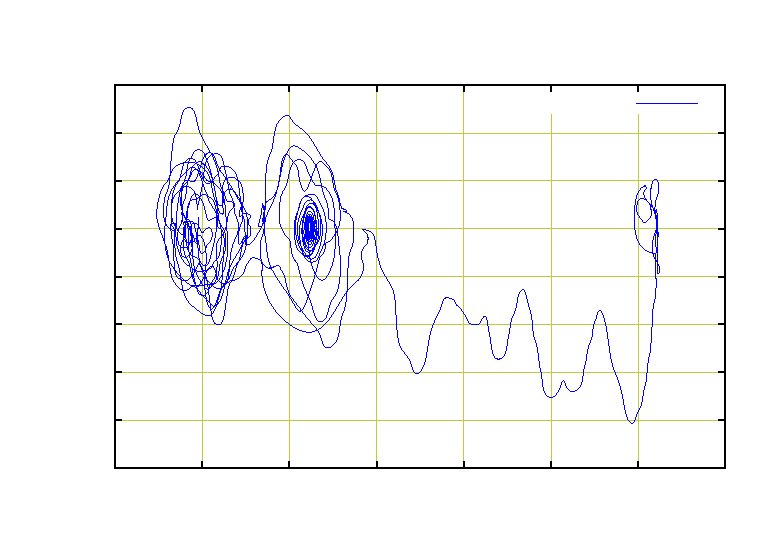
\includegraphics{eg4}}%
    \gplfronttext
  \end{picture}%
\endgroup
}
	\caption{The second bob does not have a stable orbit }
	\label{dobulepend3}
\end {figure}

\begin {figure}[!htb]
	\resizebox{\columnwidth}{!}{% GNUPLOT: LaTeX picture with Postscript
\begingroup
  \makeatletter
  \providecommand\color[2][]{%
    \GenericError{(gnuplot) \space\space\space\@spaces}{%
      Package color not loaded in conjunction with
      terminal option `colourtext'%
    }{See the gnuplot documentation for explanation.%
    }{Either use 'blacktext' in gnuplot or load the package
      color.sty in LaTeX.}%
    \renewcommand\color[2][]{}%
  }%
  \providecommand\includegraphics[2][]{%
    \GenericError{(gnuplot) \space\space\space\@spaces}{%
      Package graphicx or graphics not loaded%
    }{See the gnuplot documentation for explanation.%
    }{The gnuplot epslatex terminal needs graphicx.sty or graphics.sty.}%
    \renewcommand\includegraphics[2][]{}%
  }%
  \providecommand\rotatebox[2]{#2}%
  \@ifundefined{ifGPcolor}{%
    \newif\ifGPcolor
    \GPcolortrue
  }{}%
  \@ifundefined{ifGPblacktext}{%
    \newif\ifGPblacktext
    \GPblacktexttrue
  }{}%
  % define a \g@addto@macro without @ in the name:
  \let\gplgaddtomacro\g@addto@macro
  % define empty templates for all commands taking text:
  \gdef\gplbacktext{}%
  \gdef\gplfronttext{}%
  \makeatother
  \ifGPblacktext
    % no textcolor at all
    \def\colorrgb#1{}%
    \def\colorgray#1{}%
  \else
    % gray or color?
    \ifGPcolor
      \def\colorrgb#1{\color[rgb]{#1}}%
      \def\colorgray#1{\color[gray]{#1}}%
      \expandafter\def\csname LTw\endcsname{\color{white}}%
      \expandafter\def\csname LTb\endcsname{\color{black}}%
      \expandafter\def\csname LTa\endcsname{\color{black}}%
      \expandafter\def\csname LT0\endcsname{\color[rgb]{1,0,0}}%
      \expandafter\def\csname LT1\endcsname{\color[rgb]{0,1,0}}%
      \expandafter\def\csname LT2\endcsname{\color[rgb]{0,0,1}}%
      \expandafter\def\csname LT3\endcsname{\color[rgb]{1,0,1}}%
      \expandafter\def\csname LT4\endcsname{\color[rgb]{0,1,1}}%
      \expandafter\def\csname LT5\endcsname{\color[rgb]{1,1,0}}%
      \expandafter\def\csname LT6\endcsname{\color[rgb]{0,0,0}}%
      \expandafter\def\csname LT7\endcsname{\color[rgb]{1,0.3,0}}%
      \expandafter\def\csname LT8\endcsname{\color[rgb]{0.5,0.5,0.5}}%
    \else
      % gray
      \def\colorrgb#1{\color{black}}%
      \def\colorgray#1{\color[gray]{#1}}%
      \expandafter\def\csname LTw\endcsname{\color{white}}%
      \expandafter\def\csname LTb\endcsname{\color{black}}%
      \expandafter\def\csname LTa\endcsname{\color{black}}%
      \expandafter\def\csname LT0\endcsname{\color{black}}%
      \expandafter\def\csname LT1\endcsname{\color{black}}%
      \expandafter\def\csname LT2\endcsname{\color{black}}%
      \expandafter\def\csname LT3\endcsname{\color{black}}%
      \expandafter\def\csname LT4\endcsname{\color{black}}%
      \expandafter\def\csname LT5\endcsname{\color{black}}%
      \expandafter\def\csname LT6\endcsname{\color{black}}%
      \expandafter\def\csname LT7\endcsname{\color{black}}%
      \expandafter\def\csname LT8\endcsname{\color{black}}%
    \fi
  \fi
  \setlength{\unitlength}{0.0500bp}%
  \begin{picture}(7200.00,5040.00)%
    \gplgaddtomacro\gplbacktext{%
      \csname LTb\endcsname%
      \put(946,704){\makebox(0,0)[r]{\strut{}$-2$}}%
      \csname LTb\endcsname%
      \put(946,1163){\makebox(0,0)[r]{\strut{}$-1.5$}}%
      \csname LTb\endcsname%
      \put(946,1623){\makebox(0,0)[r]{\strut{}$-1$}}%
      \csname LTb\endcsname%
      \put(946,2082){\makebox(0,0)[r]{\strut{}$-0.5$}}%
      \csname LTb\endcsname%
      \put(946,2542){\makebox(0,0)[r]{\strut{}$0$}}%
      \csname LTb\endcsname%
      \put(946,3001){\makebox(0,0)[r]{\strut{}$0.5$}}%
      \csname LTb\endcsname%
      \put(946,3460){\makebox(0,0)[r]{\strut{}$1$}}%
      \csname LTb\endcsname%
      \put(946,3920){\makebox(0,0)[r]{\strut{}$1.5$}}%
      \csname LTb\endcsname%
      \put(946,4379){\makebox(0,0)[r]{\strut{}$2$}}%
      \csname LTb\endcsname%
      \put(1078,484){\makebox(0,0){\strut{}$-2$}}%
      \csname LTb\endcsname%
      \put(1794,484){\makebox(0,0){\strut{}$-1.5$}}%
      \csname LTb\endcsname%
      \put(2509,484){\makebox(0,0){\strut{}$-1$}}%
      \csname LTb\endcsname%
      \put(3225,484){\makebox(0,0){\strut{}$-0.5$}}%
      \csname LTb\endcsname%
      \put(3941,484){\makebox(0,0){\strut{}$0$}}%
      \csname LTb\endcsname%
      \put(4656,484){\makebox(0,0){\strut{}$0.5$}}%
      \csname LTb\endcsname%
      \put(5372,484){\makebox(0,0){\strut{}$1$}}%
      \csname LTb\endcsname%
      \put(6087,484){\makebox(0,0){\strut{}$1.5$}}%
      \csname LTb\endcsname%
      \put(6803,484){\makebox(0,0){\strut{}$2$}}%
      \put(176,2541){\rotatebox{-270}{\makebox(0,0){\strut{}y (meters)}}}%
      \put(3940,154){\makebox(0,0){\strut{}x (meters)}}%
      \put(3940,4709){\makebox(0,0){\strut{}double pendulum - full chaos}}%
    }%
    \gplgaddtomacro\gplfronttext{%
      \csname LTb\endcsname%
      \put(5816,4206){\makebox(0,0)[r]{\strut{}pendulum 1}}%
      \csname LTb\endcsname%
      \put(5816,3986){\makebox(0,0)[r]{\strut{}pendulum 2}}%
    }%
    \gplbacktext
    \put(0,0){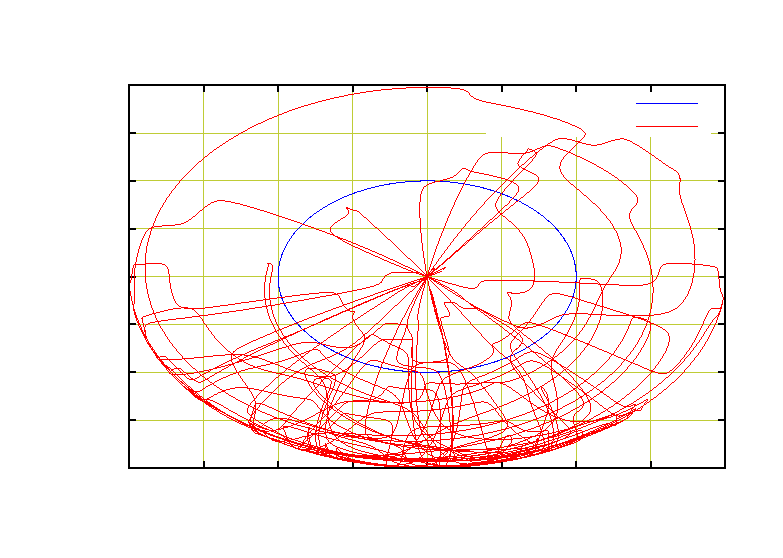
\includegraphics{eg5}}%
    \gplfronttext
  \end{picture}%
\endgroup
}
	\caption{Notice that the first pendulum spins in a full circle at times.  }
	\label{dobulepend3}
\end {figure}


\section{Summary and conclusions}

The double pendulum is a chaotic system.

\begin{thebibliography}{}


\bibitem{metcalf} M.\ Metcalf, J.\ Reid and M.\ Cohen, {\it Fortran 95/2003 explained}. Oxford University Press, 2004.
 

\end{thebibliography}




\end{document}
